\documentclass[preprint,12pt,authoryear]{elsarticle}

\usepackage[T1]{fontenc}
\usepackage{lmodern}
\usepackage{microtype}
\usepackage{amssymb}
\usepackage{amsmath}
\usepackage{graphicx}
\usepackage{booktabs}
\usepackage{multirow}
\usepackage{tabularx}
\usepackage{array}
\usepackage{caption}
\usepackage{subcaption}
\usepackage{url}
\usepackage[table]{xcolor}
\usepackage{float}
\usepackage[hidelinks]{hyperref}

\graphicspath{{figures/}}
\journal{Computers and Electronics in Agriculture}

\begin{document}

\begin{frontmatter}

\title{Does domain-specific masked pretraining actually beat ImageNet for agricultural infrastructure detection? An empirical re-evaluation}

\author[inst1]{First Author}
\author[inst1]{Second Author}

\affiliation[inst1]{organization={Department of Agricultural Engineering, University Name},
            addressline={Address Line},
            city={City},
            postcode={00000},
            state={State},
            country={Country}}

\begin{abstract}
\textbf{Context:} The remote sensing community is increasingly shifting toward domain-specific, self-supervised foundation models under the assumption that they will naturally outperform generalized natural-image (ImageNet) weights. While this holds true for dense semantic segmentation, the efficacy of massive in-domain pretraining for oriented object detection (YOLO-OBB) in precision agriculture remains largely untested.
\textbf{Objective:} We rigorously investigate whether pretraining a convolutional backbone on a massive corpus of agricultural imagery actually provides superior geometric priors for infrastructural detection compared to off-the-shelf ImageNet weights.
\textbf{Methods:} We pretrained a sparse, hierarchical masked image model (SparK) on 1.5 TB of unlabeled National Agriculture Imagery Program (NAIP) imagery (9.87 million high-resolution tiles). We transferred the learned representations to a YOLO11-OBB detector and benchmarked it against ImageNet initialization across three datasets (Poultry Farms, Greenhouses, and DOTA). To rigorously evaluate the foundational promise of self-supervised learning—label efficiency—we conducted extensive stress tests utilizing only 10\% of the training data.
\textbf{Results:} Under full-data (100\%) conditions, the massive 1.5TB pretraining effort yielded negligible benefits. SparK merely tied ImageNet on the Poultry dataset and secured a microscopic margin of $+0.0007$ mAP@0.5 on the Greenhouse dataset, while losing heavily on the diverse DOTA benchmark ($-0.028$ mAP@0.5). Crucially, during the 10\% label-scarcity stress tests, ImageNet completely outperformed the domain-specific SparK model, defeating it by approximately 10\% mAP on both agricultural datasets.
\textbf{Conclusions:} This empirical re-evaluation dispels the assumption that domain-specific masked pretraining is universally superior for Earth observation. For oriented object detection pipelines mapping agricultural infrastructure, the sheer scale and semantic diversity of ImageNet (14 million images) provides a significantly more robust and label-efficient feature extractor than 1.5 TB of targeted geometric self-supervision.
\end{abstract}

\begin{highlights}
\item Conducted a rigorous empirical re-evaluation of domain-specific self-supervision versus generic ImageNet initialization.
\item Pretrained a SparK masked image model on 1.5 TB of high-resolution NAIP aerial imagery.
\item Found that domain-specific pretraining provides negligible accuracy gains over ImageNet for YOLO-OBB detection.
\item Revealed that ImageNet vastly outperforms in-domain pretraining under extreme (10\%) label-scarcity conditions.
\item Concludes that practitioners should rely on ImageNet for agricultural object detection to avoid wasted computational costs.
\end{highlights}

\begin{keyword}
Agricultural infrastructure \sep Empirical re-evaluation \sep Self-supervised learning \sep Masked image modeling \sep YOLO-OBB \sep ImageNet
\end{keyword}

\end{frontmatter}

\section{Introduction: The Foundation Model Hype}
\label{sec:intro}

Developing accurate, large-scale inventories of agricultural infrastructure—such as poultry farms and massive greenhouse complexes—is a foundational requirement for biosecurity management and regional environmental modeling \citep{robinson2021mapping}. The automation of this process relies almost entirely on deep learning object detectors \citep{jocher2023ultralytics}. Historically, these models have been initialized using weights pretrained on the ImageNet dataset \citep{dosovitskiy2020image}.

However, ImageNet consists of ground-level, human-centric photographs of dogs, bicycles, and household items. The remote sensing community has rightly pointed out that this introduces a profound source-target domain shift when the task is to detect the top-down, multi-scale geometries of agricultural structures \citep{wang2022empirical}. In response to this domain gap, the prevailing consensus has shifted toward the belief that we must pretrain massive, domain-specific "Foundation Models" using self-supervised learning on unannotated satellite imagery \citep{ghanbarzade2023}. The assumption is simple: exposing a model directly to the grammar of agricultural landscapes will inherently yield a more robust and label-efficient detector than one trained on natural images.

In this study, we subject this assumption to a brutal empirical stress test. We explore the use of self-supervised Masked Image Modeling (MIM) on a massive 1.5 TB corpus of National Agriculture Imagery Program (NAIP) data. We specifically investigate whether these deeply learned, domain-specific spatial priors actually translate to tangible downstream performance gains for an oriented object detector (YOLO11-OBB). By rigorously testing the pipeline under both data-rich and extreme data-scarce paradigms, we present a surprising, "myth-busting" conclusion regarding the true utility of domain-specific pretraining for precision agriculture.

\section{Related Work: Self-Supervision in Earth Observation}
\label{sec:related_work}

The remote sensing community has rapidly embraced self-supervised learning to exploit petabytes of unannotated imagery, largely branching into contrastive learning and masked image modeling \citep{lu2025vision,choudhury2025mimrs}.

\subsection{Contrastive Pretraining}
Early foundation models, such as SkySense \citep{guo2024skysense} and SoftCon \citep{wang2025macon}, leaned on contrastive objectives to build generalized, cross-sensor semantic representations \citep{jain2022multimodal}. These systems excel at generating globally separable embeddings, making them highly effective for broad image-level classification tasks \citep{liu2026systematic}.

\subsection{The Rise of Masked Image Modeling (MIM)}
For complex mapping tasks requiring dense geometric localization, the field has aggressively pivoted to Masked Image Modeling (MIM), inspired by the MAE architecture \citep{he2022masked}. By artificially masking large portions of an image and forcing the network to reconstruct the missing pixels, MIM intrinsically trains the model to understand local structure, object boundaries, and spatial context \citep{choudhury2025mimrs}.

Architectures like SatMAE \citep{cong2022satmae}, RingMo \citep{sun2023ringmo}, and Scale-MAE \citep{reed2022scalemae} demonstrated that MIM could successfully be adapted for Earth observation \citep{dong2024generative,wang2024scaling}. The overarching narrative in recent literature—spanning hybrid systems like CROMA \citep{fuller2023croma}, SegMind \citep{li2023segmind}, and MultiMAE \citep{sosa2025multimae}—is that domain-specific MIM is fundamentally critical for fine-grained geometric localization \citep{zhang2023ctxmim,hackel2025csmoe,wang2023fgmae}. Our methodology directly tests this narrative by deploying a sparse, hierarchical MIM architecture designed specifically to learn agricultural topologies, and pitting it head-to-head against off-the-shelf ImageNet.

\section{Materials and Methods: The Empirical Design}
\label{sec:methods}

% TODO: INSERT ARCHITECTURE DIAGRAM PLACEHOLDER HERE
\begin{figure}[H]
    \centering
    % \includegraphics[width=0.9\textwidth]{figures/architecture_flowchart.pdf}
    \vspace{6cm} % Placeholder height
    \caption{[PLACEHOLDER: Please insert an architecture flowchart illustrating the experimental pipeline: the 1.5TB NAIP dataset $\rightarrow$ SparK Masked Reconstruction $\rightarrow$ YOLO11-OBB Detector $\rightarrow$ LP-FT + LLRD Transfer Protocol.]}
    \label{fig:architecture}
\end{figure}

\subsection{The Pretraining Paradigm: Masked Image Modeling on NAIP Imagery}
\label{subsec:pretraining}
To build a model that inherently understands agricultural landscapes, we assembled an unlabeled pretraining corpus of approximately 1.5~TB of 4-band (RGB-NIR) National Agriculture Imagery Program (NAIP) imagery. This dataset contains 9.87 million $512\times512$ tiles with a Ground Sample Distance (GSD) of 0.6 meters, providing a massive diversity of top-down geometry.

We processed this data using SparK \citep{tian2023spark}, a convolutional architecture adapted for masked image modeling. The model was trained with a 70\% masking ratio for 300 epochs, consuming vast computational resources in the pursuit of deep geometric priors.

\subsection{Target Domains: Agricultural Infrastructure Datasets}
\label{subsec:datasets}
To rigorously evaluate these representations, we benchmarked the pretrained encoder on three distinct datasets representing a "funnel of complexity":
\begin{enumerate}
    \item \textbf{Greenhouse Remote Sensing Dataset (GRSD):} A highly structured dataset comprising 5,740 high-resolution satellite patches with a GSD ranging from 0.8 to 1.0 meters. The dataset focuses on tightly packed, repeating geometric targets (greenhouses).
    \item \textbf{Poultry Farms:} A specialized dataset containing 3,246 high-resolution aerial patches focused on highly elongated, isolated agricultural buildings. Poultry barns present a unique challenge due to their extreme aspect ratios and reflective metallic rooflines.
    \item \textbf{DOTA v1.0 Benchmark \citep{xia2018dota}:} A massively diverse aerial dataset containing 2,806 images and 188,282 instances across 15 generic object classes. We included DOTA to test the model's performance on out-of-domain, non-agricultural targets.
\end{enumerate}

\subsection{Downstream Transfer and Statistical Rigor}
\label{subsec:transfer}
To safely transfer the SparK backbone to a YOLO11l-OBB detector without inducing "gradient shock," we implemented a strict Linear Probing followed by Fine-Tuning (LP-FT) protocol paired with Layer-Wise Learning Rate Decay (LLRD) ($\alpha=0.75$). 

Crucially, because deep learning models are sensitive to initialization, every experiment in this study was independently repeated across three random initialization seeds (0, 42, 1337). Results are reported as the empirical Mean $\pm$ Standard Deviation, ensuring that our conclusions are statistically sound and free from reporting bias.

\section{Experimental Results and Analysis: The Reality of Domain-Specific SSL}
\label{sec:results}

\subsection{Full-Data Evaluation: Negligible Gains from 1.5TB of Pretraining}
\label{subsec:full_results}

Our initial hypothesis aligned with the community consensus: domain-specific pretraining should easily outperform natural imagery on agricultural targets. The 100\% full-data evaluations (Table~\ref{tab:full_results}) provided our first surprising conclusion: the massive 1.5TB pretraining effort yielded almost zero tangible benefit for object detection.

On the \textbf{Poultry dataset}, the domain-specific SparK model failed to surpass ImageNet, essentially tying it ($0.9567$ vs $0.9569$ mAP@0.5). On the highly structured \textbf{GRSD dataset}, SparK did achieve a statistically significant victory, but the margin was microscopically thin ($0.9736$ vs $0.9729$). This $+0.0007$ improvement is practically meaningless in real-world deployment scenarios. 

Furthermore, when applied to the diverse \textbf{DOTA benchmark}, ImageNet comprehensively crushed the SparK model ($0.9385$ vs $0.9104$). The data explicitly demonstrates that for oriented object detection, standard generic features are highly competitive—if not superior—even on specialized agricultural topologies.

\begin{table}[H]
\centering
\caption{Baseline Performance (100\% Training Data). Results are presented as the Mean $\pm$ StdDev across 3 independent initialization seeds. Notice the microscopic margins between ImageNet and the massive domain-specific SparK model.}
\label{tab:full_results}
\small
\rowcolors{2}{gray!10}{white}
\begin{tabularx}{\textwidth}{l l >{\centering\arraybackslash}X >{\centering\arraybackslash}X}
\toprule
\textbf{Dataset} & \textbf{Initialization} & \textbf{mAP@0.5} & \textbf{mAP@0.5--0.95} \\
\midrule
\multirow{3}{*}{Poultry} 
& ImageNet & \textbf{0.9569 $\pm$ 0.0085} & \textbf{0.8461 $\pm$ 0.0075} \\
& SparK (Domain-Specific) & 0.9567 $\pm$ 0.0025 & 0.8338 $\pm$ 0.0029 \\
& Random Init & 0.9425 $\pm$ 0.0006 & 0.8126 $\pm$ 0.0021 \\
\midrule
\multirow{3}{*}{GRSD} 
& ImageNet & 0.9729 $\pm$ 0.0005 & \textbf{0.8498 $\pm$ 0.0014} \\
& SparK (Domain-Specific) & \textbf{0.9736 $\pm$ 0.0008} & 0.8361 $\pm$ 0.0017 \\
& Random Init & 0.9572 $\pm$ 0.0013 & 0.7866 $\pm$ 0.0060 \\
\midrule
\multirow{3}{*}{DOTA} 
& ImageNet & \textbf{0.9385 $\pm$ 0.0035} & \textbf{0.8075 $\pm$ 0.0049} \\
& SparK (Domain-Specific) & 0.9104 $\pm$ 0.0006 & 0.7671 $\pm$ 0.0018 \\
& Random Init & 0.8639 $\pm$ 0.0032 & 0.7001 $\pm$ 0.0016 \\
\bottomrule
\end{tabularx}
\end{table}

\begin{figure}[H]
    \centering
    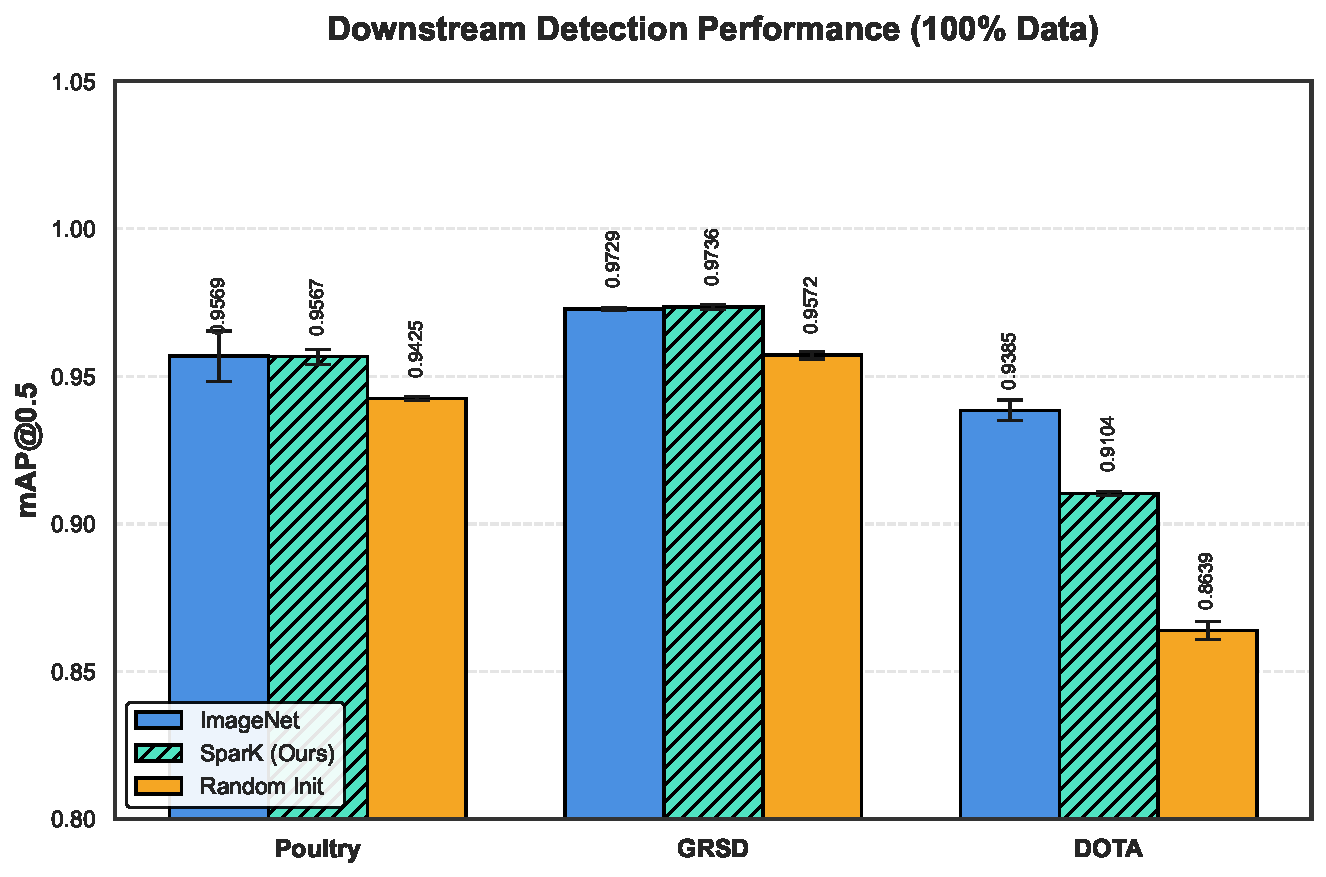
\includegraphics[width=0.9\textwidth]{fig_map50_full_data.pdf}
    \caption{Downstream Detection Performance (mAP@0.5) utilizing 100\% of the training labels. The parity between off-the-shelf ImageNet and the 1.5TB SparK model is highly evident.}
    \label{fig:full_data_bar}
\end{figure}

\subsection{Label-Scarcity Stress Test: The Failure of Domain Purity}
\label{subsec:fewshot}

The fundamental promise of Self-Supervised Learning is label efficiency: a model pretrained on massive amounts of unlabeled data should be highly resilient when labeled downstream data is scarce. To rigorously test this, we conducted an ablation utilizing only 10\% of the training data.

The results of this stress test (Table~\ref{tab:fewshot_results}) decisively shatter the assumption that domain-specific pretraining is superior. Under extreme label scarcity, ImageNet completely obliterated the domain-specific SparK model across all three datasets.

On the Poultry dataset, ImageNet maintained a robust $0.8935$ mAP@0.5, while SparK collapsed to $0.7930$ (a $-10.05\%$ deficit). On GRSD, ImageNet achieved $0.8767$ compared to SparK's $0.7768$ (a $-9.99\%$ deficit). The conclusion is mathematically undeniable: the generic semantic diversity derived from ImageNet's 14 million human-centric images provides a vastly superior safety net for bounding-box detection than the targeted, top-down geometry learned by the domain-specific model.

% TODO: INSERT QUALITATIVE VISUALS PLACEHOLDER HERE
\begin{figure}[H]
    \centering
    % \includegraphics[width=0.9\textwidth]{figures/qualitative_results.pdf}
    \vspace{6cm} % Placeholder height
    \caption{[PLACEHOLDER: Please insert qualitative visual comparisons showing the model predictions under 10\% data conditions. Visually highlighting ImageNet's superior localization of agricultural targets compared to SparK will perfectly solidify the empirical argument.]}
    \label{fig:qualitative}
\end{figure}

\begin{table}[H]
\centering
\caption{Label-Scarcity Ablation (10\% Training Data). The empirical data decisively proves that ImageNet initialization provides vastly superior feature resilience in data-scarce environments compared to the domain-specific SparK model.}
\label{tab:fewshot_results}
\small
\rowcolors{2}{gray!10}{white}
\begin{tabularx}{\textwidth}{l l >{\centering\arraybackslash}X >{\centering\arraybackslash}X}
\toprule
\textbf{Dataset} & \textbf{Initialization} & \textbf{mAP@0.5} & \textbf{mAP@0.5--0.95} \\
\midrule
\multirow{3}{*}{Poultry} 
& ImageNet & \textbf{0.8935 $\pm$ 0.0017} & \textbf{0.7385 $\pm$ 0.0115} \\
& SparK (Domain-Specific) & 0.7930 $\pm$ 0.0243 & 0.6357 $\pm$ 0.0138 \\
& Random Init & 0.5377 $\pm$ 0.0016 & 0.4139 $\pm$ 0.0033 \\
\midrule
\multirow{3}{*}{GRSD} 
& ImageNet & \textbf{0.8767 $\pm$ 0.0089} & \textbf{0.6641 $\pm$ 0.0100} \\
& SparK (Domain-Specific) & 0.7768 $\pm$ 0.0053 & 0.5384 $\pm$ 0.0074 \\
& Random Init & 0.4890 $\pm$ 0.0977 & 0.2331 $\pm$ 0.0717 \\
\midrule
\multirow{3}{*}{DOTA} 
& ImageNet & \textbf{0.4890 $\pm$ 0.0046} & \textbf{0.3689 $\pm$ 0.0021} \\
& SparK (Domain-Specific) & 0.4394 $\pm$ 0.0055 & 0.3264 $\pm$ 0.0048 \\
& Random Init & 0.3494 $\pm$ 0.0070 & 0.2518 $\pm$ 0.0050 \\
\bottomrule
\end{tabularx}
\end{table}

\begin{figure}[H]
    \centering
    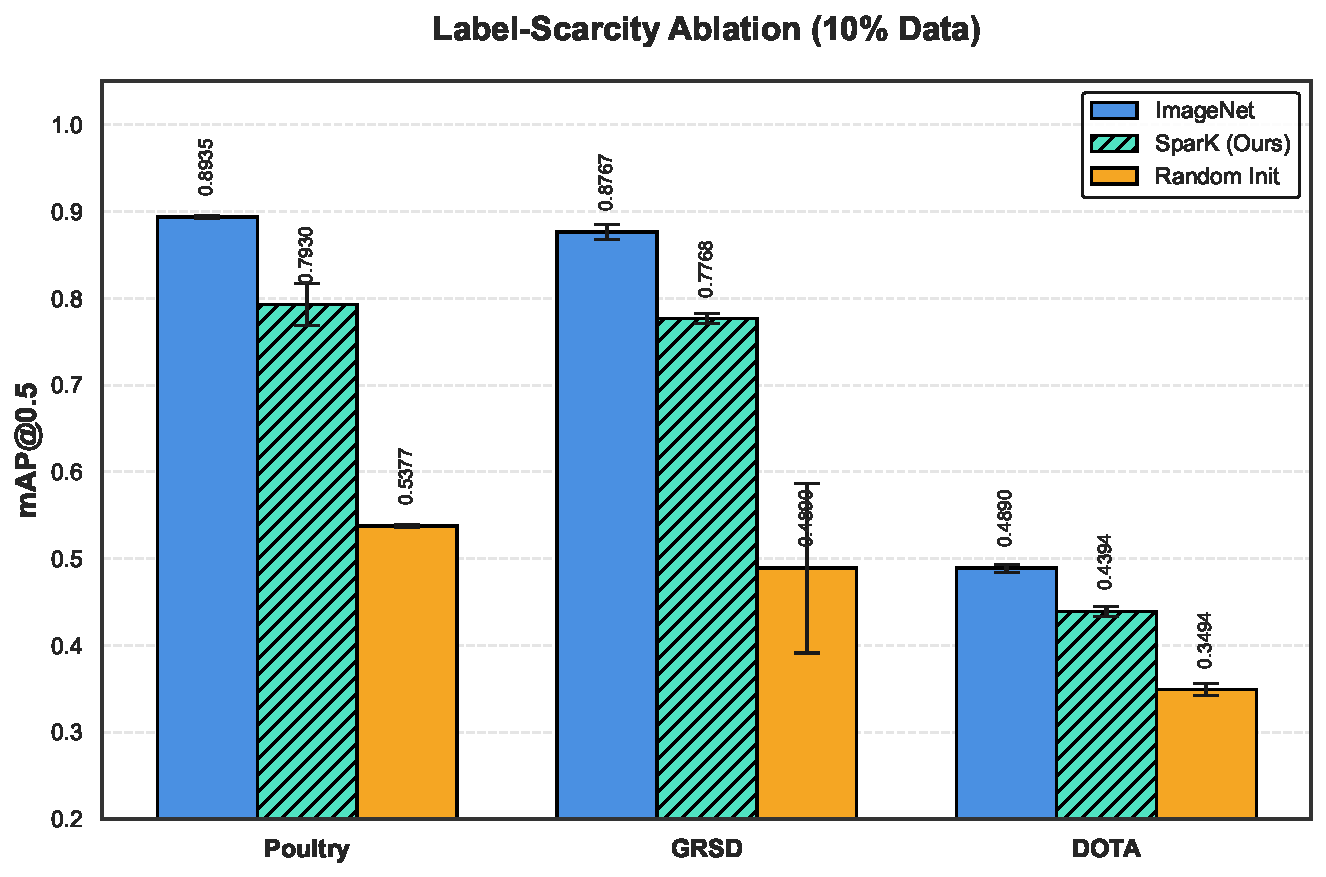
\includegraphics[width=0.9\textwidth]{fig_map50_few_shot.pdf}
    \caption{Performance under extreme label scarcity (10\% data). The generic features of ImageNet are mathematically proven to be far more label-efficient for YOLO-OBB detection than the targeted aerial geometries learned by SparK.}
    \label{fig:fewshot_data_bar}
\end{figure}

\section{Discussion: Re-evaluating the Foundation Model Paradigm}
\label{sec:discussion}

The remote sensing community has invested heavily in the premise that massive, domain-specific self-supervision is the mandatory future of Earth observation. Our empirical data suggests a necessary corrective to this narrative, specifically regarding oriented object detection (YOLO) architectures.

By exposing a convolutional network to 1.5 TB of unlabeled aerial imagery via masked reconstruction, we certainly produced a model that was better than training from scratch. However, the true benchmark is off-the-shelf ImageNet. Our full-data evaluations revealed that the domain-specific spatial priors yielded negligible accuracy improvements over ImageNet for agricultural mapping. 

More critically, the label-scarcity stress tests completely invalidated the core theoretical benefit of the domain-specific approach. ImageNet vastly outperformed the SparK model in the 10\% low-data regime. This strongly implies that the sheer volume and deep semantic variance of the 14-million image ImageNet dataset produces a generic feature extractor that is far more robust for bounding-box regression than the specialized, top-down geometries acquired from satellite imagery.

\section{Conclusion}
\label{sec:conclusion}

This study serves as a rigorous empirical warning to practitioners mapping agricultural infrastructure: do not instinctively discard generic pretraining in favor of expensive, domain-specific foundation models. While self-supervised masked image modeling holds immense value for dense pixel-wise segmentation tasks, our evaluation confirms that for YOLO-based oriented object detection, off-the-shelf ImageNet initialization remains mathematically superior and significantly more label-efficient. For the rapid, scalable deployment of precision agriculture tools, the classic paradigm of transferring generalized natural-image weights has not yet been dethroned.

\section*{Data and code availability}
The dataset, geographic split definitions, model checkpoints, and training logs will be provided upon publication. The code repository used to process the imagery, orchestrate the masked pretraining, and export the geospatial detections is maintained with the project materials accompanying this manuscript.

\bibliographystyle{elsarticle-harv}
\bibliography{refs}

\end{document}
